\begin{figure}[t]
\uwsinglespace
\begin{center}
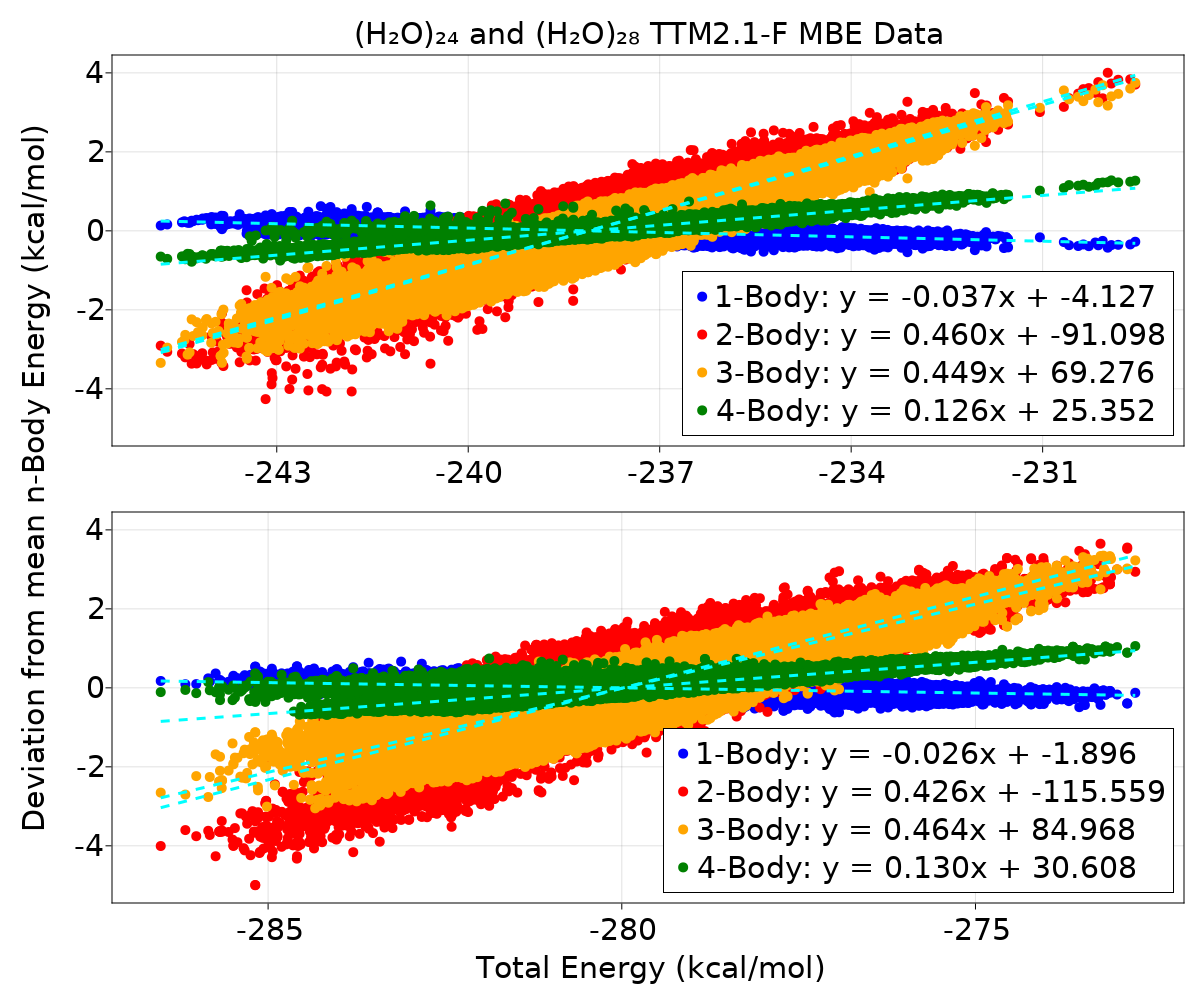
\includegraphics[width=.8\textwidth]{Figures/Chapter_6/w24_and_w28_mbe_ttm21f_deviation.png}
\end{center}
\begin{spacing}{1.0}
\caption[Panels for \ce{(H2O)_{24}} (top) and \ce{(H2O)_{28}} (bottom), showing the deviation of each many-body term $E_{nB}$ from the average of the same many-body term, $\langle E_nB\rangle$, plotted against the total energy for a cluster. Notice that the slope of each line is the percentage contribution to the binding energy.]{Panels for \ce{(H2O)_{24}} (top) and \ce{(H2O)_{28}} (bottom), showing the deviation of each many-body term $E_{nB}$ from the average of the same many-body term, $\langle E_nB\rangle$, plotted against the total energy for a cluster. Notice that the slope of each line is the percentage contribution to the binding energy.}\label{fig:MBE_III_F5}
\end{spacing}
\end{figure}